Volem construir una peça metàl·lica que tingui per secció un trapezi isòsceles amb la base superior tres vegades
més llarga que la base inferior. Els altres costats del trapezi fan 10 mm, tal com podeu observar en la figura
següent:
\begin{center}
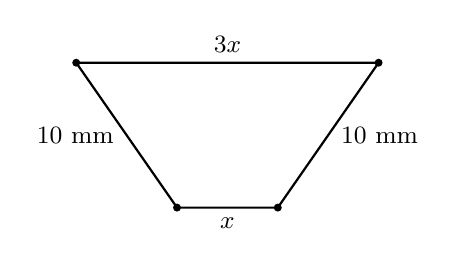
\begin{tikzpicture}[scale=0.8]
  \draw[thick] (0,2.3) -- (4.8,2.3) -- (3.2,0) -- (1.6,0) -- cycle;
  \foreach \p in {(0,2.3),(4.8,2.3),(3.2,0),(1.6,0)} \fill \p circle (1.8pt);
  \node[above,font=\small] at (2.4,2.3) {$3x$};
  \node[below,font=\small] at (2.4,0) {$x$};
  \node[left,font=\small] at (0.75,1.15) {10 mm};
  \node[right,font=\small] at (4.05,1.15) {10 mm};
\end{tikzpicture}
\end{center}

\begin{apartats}

\apartat{0,5}
Expresseu l'altura del trapezi en funció de la longitud $x$ de la base inferior.

\begin{solucio}
A partir de la situació exposada, tenim el gràfic següent:
\begin{center}
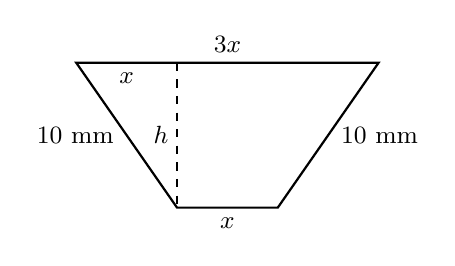
\begin{tikzpicture}[scale=0.8]
  \draw[thick] (0,2.3) -- (4.8,2.3) -- (3.2,0) -- (1.6,0) -- cycle;
  \draw[dashed] (1.6,2.3) -- (1.6,0);
  \node[above,font=\small] at (2.4,2.3) {$3x$};
  \node[below,font=\small] at (0.8,2.3) {$x$};
  \node[left,font=\small] at (1.62,1.15) {$h$};
  \node[below,font=\small] at (2.4,0) {$x$};
  \node[left,font=\small] at (0.75,1.15) {10 mm};
  \node[right,font=\small] at (4.05,1.15) {10 mm};
\end{tikzpicture}
\end{center}
Pel teorema de Pitàgores, s'obté que $x^2+h^2=10^2$ i, per tant, $\boxed{h=\sqrt{100-x^2}}$.

\textit{Pauta oficial:} 0,25 per l'aplicació del teorema de Pitàgores i 0,25 per l'expressió final.
\end{solucio}

\apartat{2}
Calculeu la longitud de la base inferior del trapezi de manera que l'àrea de la peça sigui màxima i trobeu el
valor d'aquesta àrea màxima.

\begin{solucio}
L'àrea del trapezi és $A(x)=\dfrac{x+3x}{2}\cdot h=2x\cdot\sqrt{100-x^2}$. Per trobar els candidats a valors que fan
màxima aquesta àrea, calcularem la funció derivada, $A'(x)$, i obtindrem les solucions de l'equació $A'(x)=0$:
\begin{align*}
A'(x)&=2\cdot\sqrt{100-x^2}+2x\cdot\frac{1}{2\sqrt{100-x^2}}\,(-2x)
=2\sqrt{100-x^2}+\frac{-2x^2}{\sqrt{100-x^2}}\\
&=\frac{2\left(100-x^2\right)-2x^2}{\sqrt{100-x^2}}=\frac{200-4x^2}{\sqrt{100-x^2}}=\frac{4\left(50-x^2\right)}{\sqrt{100-x^2}}.
\end{align*}
Per tant, tindrem $A'(x)=0$ quan $50-x^2=0$, és a dir, $x^2=50$ i $x=\pm\sqrt{50}=\pm5\sqrt2\approx\pm7{,}07$. A
partir del context de l'enunciat, l'únic candidat és el valor positiu, $x=\sqrt{50}=7{,}07$ mm. Ara cal comprovar
que amb aquest valor l'àrea és màxima, i això es comprova veient que per a valors propers l'àrea és més petita:
\[
A(7)=99{,}980,\qquad A\!\left(\sqrt{50}\right)=2\cdot\sqrt{50}\cdot\sqrt{100-50}=2\cdot\sqrt{50}\cdot\sqrt{50}=100,\qquad
A(7{,}1)=99{,}9966 .
\]
Per tant, el valor de la base petita que fa l'àrea màxima és de $5\sqrt2=7{,}07$ mm, i el valor de l'àrea és de
$100\ \text{mm}^2$. Per comprovar la condició de màxim, també es podria veure que la derivada segona de la funció
àrea és negativa per al valor $x=\sqrt{50}$.

\textit{Pauta oficial:} 0,25 per la formulació de l'àrea del trapezi, 0,25 per l'expressió de l'àrea en funció de
$x$, 0,5 per la derivada de la funció, 0,25 pel càlcul del punt singular, 0,5 per l'avaluació de la condició de
màxim relatiu i 0,25 pel càlcul de l'àrea màxima.
\end{solucio}

\end{apartats}
